
\section*{Основания для разработки}
Разработка ведётся в рамках выполнения лабораторных работ по курсу <<Методология программной инженерии>> на кафедре <<Программное обеспечение ЭВМ и информационные технологии>> факультета <<Информатика и системы управления>> МГТУ им. Н.Э. Баумана.

\section*{Назначение разработки}
Разрабатываемая система должна предоставлять пользователям возможность бронирования номеров сети Apartlux, в которую входят 14 гостиниц в Москве на таких станциях метро, как Бабушкинская, Рижская, Тверская, Авиамоторная и другие. Должен быть предусмотрен поиск подходящих номеров по таким параметрам, как этаж, дата и продолжительность бронирования, стоимость, число мест, наличие двуспальной кровати. В зависимости от количества сделанных ранее заказов система должна рассчитывать скидку на новые согласно условиям программы лояльности.

\section*{Существующие аналоги}
У сети Apartlux уже есть действующий с 2011 года сайт для бронирования, который имеет ряд недостатков. При его создании разработчики придерживались подходам монолитной архитектуры, поэтому сейчас компания столкнулась с такими трудностями, как:
\begin{enumerate}
	\item проблематичность масштабирования;
	
	\item сложность внедрения появившихся технологий, которые используются повсеместно;
	
	\item внесение даже незначительного изменения в функциональность существенно усложняет и замедляет разработку.
\end{enumerate}

В то время как на российском рынке гостиничных услуг появляется всё больше компаний, например, Radisson, Azimut Hotels, Hilton, остановивших свой выбор на микросервисной архитектуре и внедряющих современные технологии: PostgreSQL, MongoDB, Kafka, ELK stack и т.д. У приведённых сетей отелей и гостиниц есть общий недостаток: непрозрачная программа лояльности, которая направлена лишь на ограниченный круг лиц.

По сравнению с существующим сайтом и указанными аналогами разрабатываемый проект должен иметь следующие преимущества:
\begin{enumerate}
	\item в основе должна лежать микросервисная архитектура, решающая сложности с масштабированием, обслуживанием и внесением изменений в функциональность;
	
	\item понятная бонусная программа, ориентированная на каждого из клиентов.
\end{enumerate}

\section*{Описание системы}
Разрабатываемый сервис должен представлять собой распределённую систему для бронирования номеров гостиниц сети Apartlux. Если клиент хочет оформить бронь, ему необходимо зарегистрироваться, указ информацию: фамилия, имя, отчество, дата рождения, номер телефона, электронная почта. В случае, если зарегистрированному ранее пользователю нужно отменить заказ, получить информацию о его бронированиях или статусе в программе лояльности, ему нужно авторизоваться. Для неавторизованных пользователей доступен только просмотр общей информации. 
На рисунке \ref{fig:schema} отображена схема предметной области.
\begin{figure}[h]
	\begin{center}
		{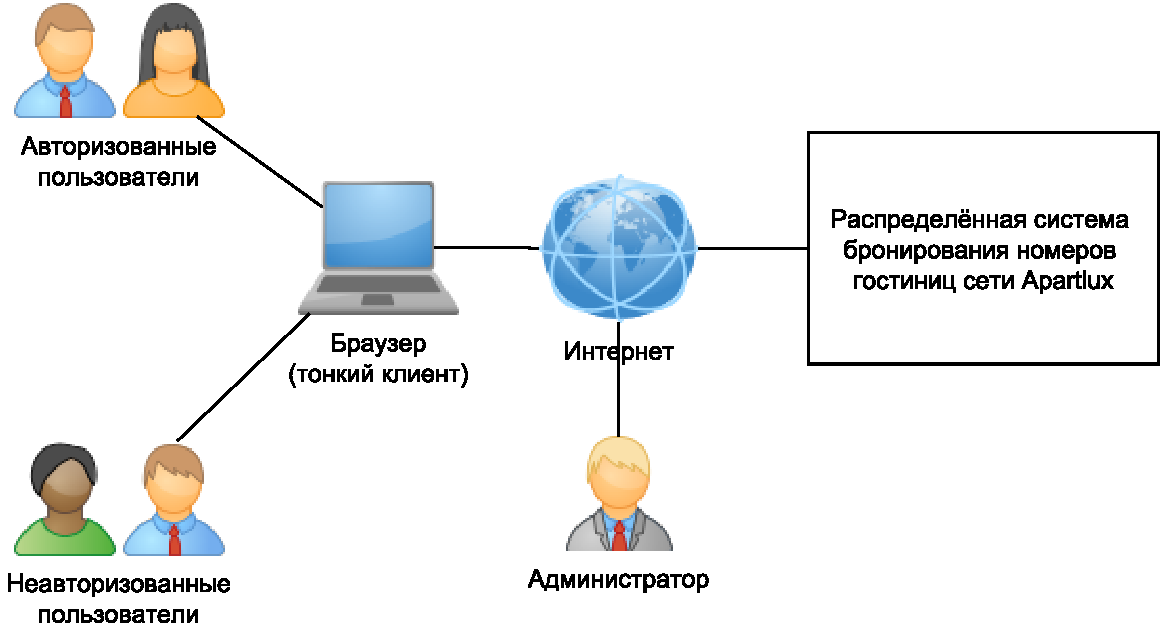
\includegraphics[scale = 0.6]{img/pic/general.pdf}}
		\caption{Схема предметной области.}
		\label{fig:schema}
	\end{center}
\end{figure}

\pagebreak

\section*{Общие требования к системе}
Требования к системе следующие.
\begin{enumerate}
	\item Разрабатываемое ПО должно поддерживать функционирование системы в режиме 24 часов, 7 дней в неделю, 365 дней в году (24/7/365) со среднегодовым временем доступности не менее 99.9\%. Допустимое время, в течении которого система недоступна, за год должна составлять $24\cdot365\cdot0.001=8.76$ ч.
	
	\item Время восстановления системы после сбоя не должно превышать 15 минут.
	
	\item Каждый узел должен автоматически восстанавливаться после сбоя.
	
	\item Система должна поддерживать возможность <<горячего>> переконфигурирования системы. Необходимо предусмотреть поддержку добавления нового узла во время работы системы без рестарта.
	
	\item Обеспечить безопасность работоспособности за счёт отказоустойчивости узлов.
\end{enumerate}

\section*{Требования к функциональным характеристикам}
\begin{enumerate}
	\item По результатам работы модуля сбора статистики медиана времени отклика системы на запросы пользователя на получение информации не должна превышать 3 секунд.
	
	\item По результатам работы модуля сбора статистики медиана времени отклика системы на запросы, добавляющие или изменяющие информацию на портале не должна превышать 7 секунд.
	
	\item Медиана времени отклика системы на действия пользователя должна быть менее 0.8 секунд при условии работы на рекомендованной аппаратной конфигурации, задержках между взаимодействующими сервисами менее 0.2 секунды и одновременном числе работающих пользователей менее 100 на каждый сервер, обслуживающий внешний интерфейс.
	
	\item Система должна обеспечивать возможность запуска в современных браузерах: не менее 85\% пользователей Интернета должны пользоваться ей без какой-либо деградации функционала.
\end{enumerate}

\section*{Функциональные требования к системе с точки зрения пользователя}
Система должна обеспечивать реализацию следующих функций.
\begin{enumerate}
	\item Регистрация и авторизация пользователей с валидацией вводимых данных как через интерфейс приложения, так и через	социальные сети.
	
	\item Аутентификация пользователей.
	
	\item Разделение всех пользователей на три роли:
	\begin{itemize}
		\item Пользователь (неавторизированный пользователь);
		
		\item Клиент (авторизированный пользователь);
		
		\item Администратор.
	\end{itemize}
	
	\item Предоставление возможностей \textbf{Пользователю, Клиенту, Администратору} представленных в таблице \ref{tbl:user-func}.
\end{enumerate}

\begin{longtable}{|p{0.5cm}|p{15.5cm}|}
	\caption{Функции пользователей}
	\label{tbl:user-func} \\
	\hline
	
	\begin{rotatebox}[origin=r]{90}
		{ \textbf{Пользователь}}
	\end{rotatebox} 
	& 
	1. просмотр списка гостиниц, входящих в сеть; \newline
	2. просмотр информации о возможности бронирования номера гостиницы по заданным реквизитам; \newline
	3. получение информации об условиях программы лояльности; \newline
	4. регистрация в системе; \newline
	5. авторизация в системе; \\
	\hline
	
	\begin{rotatebox}[origin=r]{90}
		{ \textbf{Клиент}}
	\end{rotatebox} 
	& 
	1. просмотр списка гостиниц, входящих в сеть; \newline
	2. просмотр информации о возможности бронирования номера гостиницы по заданным реквизитам; \newline
	3. получение информации об условиях программы лояльности; \newline
	4. авторизация в системе; \newline
	5. получение и изменение информации текущего аккаунта; \newline
	6. просмотр всех бронирований, зарегистрированных на имя текущего клиента; \newline
	7. получение детальной информации по конкретному бронированию текущего клиента; \newline
	8. бронирование отеля на имя текущего клиента; \newline
	9. отмена заказа, оформленного на имя текущего пользователя; \newline
	10. получение информации о статусе текущего пользователя в программе лояльности. \\
	\hline
	
	\begin{rotatebox}[origin=r]{90}
	{ \textbf{Администратор}}
	\end{rotatebox} 
	& 
	1. просмотр списка гостиниц, входящих в сеть; \newline
	2. просмотр информации о возможности бронирования номера гостиницы по заданным реквизитам; \newline
	3. получение информации об условиях программы лояльности; \newline
	4. авторизация в системе; \newline
	5. получение и редактирование информации о любом клиенте, зарегистрированном в системе; \newline
	6. просмотр и редактирование всех оформленных бронирований; \newline
	7. получение детальной информации по конкретному бронированию; \newline
	8. бронирование отеля на зарегистрированного в системе пользователя; \newline
	9. отмена любого оформленного заказа; \\
	&
	10. получение информации о статусе в программе лояльности любого зарегистрированного в системе клиента; \newline
	11. изменение доступных дат для бронирования; \newline
	12. редактирование информации об условиях программы лояльности. \\	
	\hline
\end{longtable}

\section*{Входные данные}
Входные параметры системы представлены в таблице \ref{tbl:input}.

\begin{longtable}{|p{3cm}|p{13cm}|}
	\caption{Входные данные}
	\label{tbl:input} \\
	\hline
	
	\textbf{Сущность} & \textbf{Входные данные} \\
	\hline
	\endfirsthead
	
	\hline
	\textbf{Сущность} & \textbf{Входные данные} \\
	\hline
	\endhead
	
	\hline
	\multicolumn{2}{c}{\textit{Продолжение на следующей странице}}
	\endfoot
	\hline
	\endlastfoot
	
	Клиент / Администратор
	&
	1. \textit{фамилия, имя} и \textit{отчество} не более 256 символов каждое поле; \newline
	2. \textit{дата рождения} в формате д/м/гггг; \newline
	3. \textit{логин} не менее 10 символов и не более 128; \newline
	4. \textit{пароль} не менее 8 символов и не более 128, как минимум одна заглавная и одна строчная буква, только латинские буквы, без пробелов, как минимум одна цифра; \newline
	5. \textit{номер телефона}; \newline
	6. \textit{электронная почта}; \\
	\hline
	
	Гостиница
	& 
	1. \textit{идентификатор}; \newline
	2. \textit{название} не более 256 символов; \newline
	3. \textit{страна}; \newline
	4. \textit{город}; \newline
	5. \textit{полный адрес} не более 1024 символа; \newline
	6. \textit{контактный телефон}; \newline
	7. \textit{электронная почта}; \newline
	8. \textit{описание} не более 2048 символов \newline
	9. \textit{количество звёзд} \\
	\hline
	
	Номер
	& 
	1. \textit{идентификатор}; \newline
	2. \textit{идентификатор} соответствующей \textit{гостиницы}; \newline
	3. \textit{число мест}; \newline
	4. \textit{этаж}; \newline
	5. \textit{стоимость}; \newline
	6. \textit{наличие двуспальной кровати}; \\
	\hline
	
	Бронирование
	&
	1. \textit{идентификатор}; \newline
	2. \textit{логин клиента}, на которое оно оформлено; \newline
	3. \textit{идентификатор гостиницы}; \newline
	4. \textit{идентификатор} соответствующей \textit{платёжной операции}; \newline
	5. \textit{статус} (APPROVED/UNAPPROVED); \newline
	6. \textit{дата въезда}; \newline
	7. \textit{дата выезда}; \\
	\hline
	
	Оплата
	& 
	1. \textit{идентификатор}; \newline
	2. \textit{фамилия, имя, отчество} человека, совершившего операцию; \newline
	3. \textit{статус} (PAID/CANCELED); \newline
	4. \textit{сумма}; \newline
	5. \textit{дата и время}.
\end{longtable}
 
 
\section*{Выходные параметры}
Выходными параметрами системы являются web-страницы. В зависимости от запроса и текущей роли пользователя  они содержат следующую информацию (таблица \ref{tbl:output-data}).

\begin{longtable}{|p{0.5cm}|p{15.5cm}|}
	\caption{Выходные параметры}
	\label{tbl:output-data} \\
	\hline
	
	\begin{rotatebox}[origin=r]{90}
		{ \textbf{Пользователь}}
	\end{rotatebox} 
	& 
	1. список гостиниц, которые входят в сеть Apartlux, указывается: \newline
	• \textit{название}; \newline
	• \textit{полный адрес}; \newline
	• \textit{описание}; \newline
	• контактная информация: \textit{телефон} и \textit{электронная почта}; \newline
	• доступные для бронирования \textit{номера} по заданным реквизитам; \\
	\cline{2-2}
	&
	2. информация об условиях текущей программы лояльности; \\
	\hline
	
	\begin{rotatebox}[origin=r]{90}
		{ \textbf{Клиент}}
	\end{rotatebox} 
	& 
	1. список гостиниц, которые входят в сеть Apartlux, указывается: \newline
	• \textit{название}; \newline
	• \textit{полный адрес}; \newline
	• \textit{описание}; \newline
	• контактная информация: \textit{телефон} и \textit{электронная почта}; \newline
	• доступные для бронирования \textit{номера} по заданным реквизитам; \\
	\cline{2-2}
	
	&
	2. информация об условиях текущей программы лояльности; \\
	\cline{2-2}
	
	&
	3. детальная информация о пользователе, вошедшем в систему; \newline
	• \textit{фамилия, имя, отчество}; \newline
	• \textit{дата рождения}; \newline
	• \textit{логин}; \newline
	• \textit{номер телефона}; \newline
	• \textit{электронная почта}; \newline
	• \textit{размер скидки}; \\
	\cline{2-2}
	
	&
	4. список оформленных бронирований на пользователя, вошеднего в систему, предоставляется информация о: \newline
	• \textit{дате въезда/выезда}; \newline
	• \textit{полный адрес} гостиницы и \textit{контактные данные}; \newline
	• информация о номере: \textit{этаж}, \textit{номер}, \textit{количество мест}; \newline
	• \textit{статус оплаты}; \newline
	• \textit{статус бронирования}; \newline
	• \textit{сумма}; \\
	\hline
	
	\begin{rotatebox}[origin=r]{90}
		{ \textbf{Администратор}}
	\end{rotatebox} 
	& 
	1. список гостиниц, которые входят в сеть Apartlux, указывается: \newline
	• \textit{название}; \newline
	• \textit{полный адрес}; \newline
	• \textit{описание}; \newline
	• контактная информация: \textit{телефон} и \textit{электронная почта}; \newline
	• доступные для бронирования \textit{номера} по заданным реквизитам; \\
	\cline{2-2}
	
	&
	2. информация об условиях текущей программы лояльности; \\
	\cline{2-2}
	
	&
	3. детальная информация о пользователе, вошедшем в систему; \newline
	• \textit{фамилия, имя, отчество}; \newline
	• \textit{дата рождения}; \newline
	• \textit{логин}; \newline
	• \textit{номер телефона}; \newline
	• \textit{электронная почта}; \newline
	• \textit{размер скидки}; \\
	\cline{2-2}
	
	&
	4. список оформленных бронирований, предоставляются такие данные, как: \newline
	• \textit{идентификатор}; \newline
	• информация о клиенте, на которое оно оформлено: \textit{логин, номер телефона, электронная почта}; \newline
	• \textit{дата въезда/выезда}; \newline
	• информация о гостинице: её \textit{идентификатор, полный адрес} и \textit{контактные данные}; \newline
	• информация о номере: \textit{этаж, номер, количество мест}; \newline	
	• информация об оплате: \textit{идентификатор, статус, ФИО оплатившего, дата} и \textit{время операции}; \newline
	• \textit{статус бронирования}; \newline
	• \textit{сумма}; \\
	\cline{2-2}
	
	&
	5. список зарегистрированных в системе клиентов с указанием: \newline
	• \textit{ФИО}; \newline
	• \textit{логина}; \newline
 	• \textit{даты рождения}; \newline
	• \textit{контактных данных}; \newline
	• \textit{персональной скидки}; \newline
	• \textit{число предыдущих бронирований}. \\
	\hline
\end{longtable}

\section*{Топология Системы}
На рисунке \ref{fig:topology} изображён один из возможных вариантов  топологии разрабатываемой распределенной Системы.
\begin{figure}[h]
	\begin{center}
		{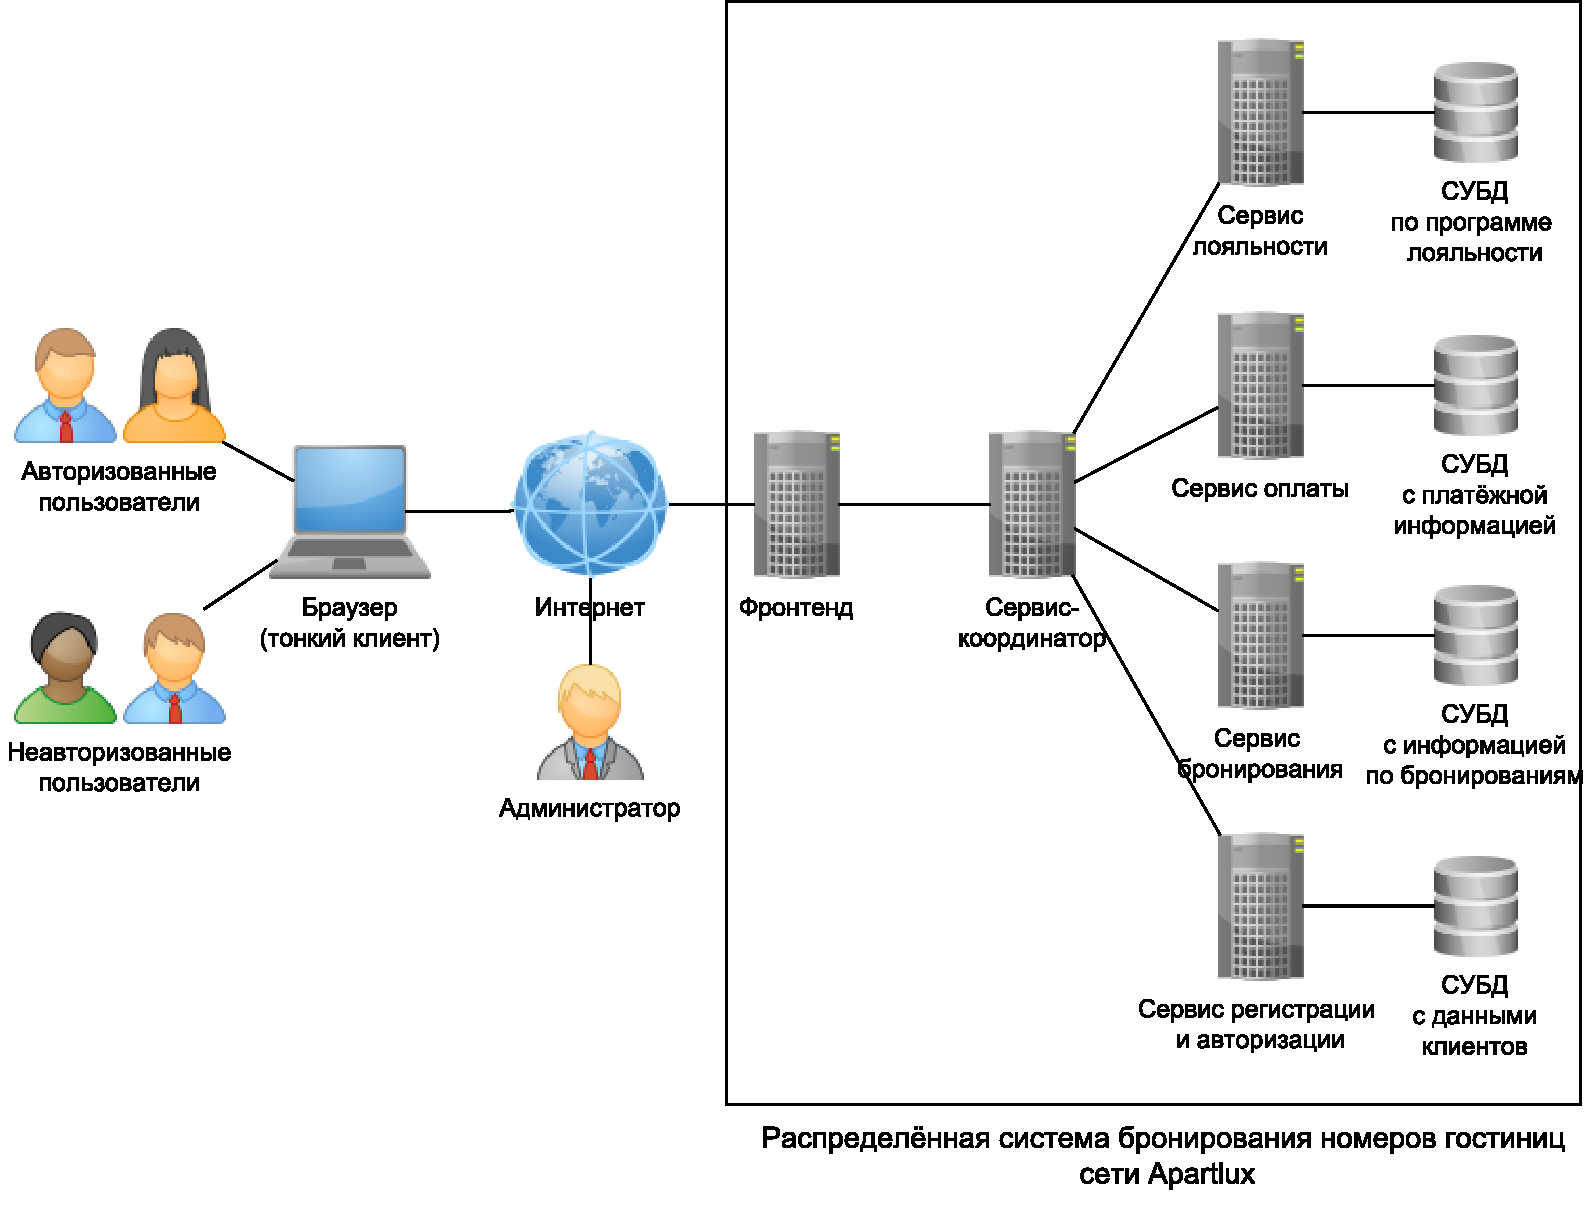
\includegraphics[scale = 0.6]{img/pic/topology.pdf}}
		\caption{Топология системы.}
		\label{fig:topology}
	\end{center}
\end{figure}

\pagebreak
%
Система будет состоять из фронтенда и 5 подсистем:
\begin{itemize}
	\item сервис-координатор;
	
	\item сервис регистрации и авторизации;
	
	\item сервис бронирования;
	
	\item сервис оплаты;
	
	\item сервис лояльности.
\end{itemize}
%
\textbf{Фротенд} принимает запросы от пользователей по протоколу HTTP и анализирует их. На основе проведенного анализа выполняет запросы к микросервисам бекенда, агрегирует ответы и отсылает их пользователю. \\
\textbf{Сервис-координатор} -- единая точка входа и межсервисной коммуникации. \\
\textbf{Сервис-регистрации и авторизации} отвечает за:
\begin{itemize}
	\item возможность регистрации нового клиента;
	
	\item аутентификацию пользователя (клиента и администратора);
	
	\item авторизацию пользователя;
	
	\item выход из сессии.
\end{itemize}
\textbf{Сервис бронирования} реализует следующие функции:
\begin{itemize}
	\item получение списка всех гостиниц, входящий в сеть Apartlux;
	
	\item получение информации о конкретной гостинице;
	
	\item получение, создание, отзыв бронирования.
\end{itemize}
\textbf{Сервис оплаты} реализует функции:
\begin{itemize}
	\item проведение платежа от клиента к системе;
	
	\item получение статуса оплаты;
	
	\item отмену платежа.
\end{itemize}
\textbf{Сервис лояльности} отвечает за ведение статистики по количеству бронирований всех клиентов, на основе которой для каждого пользователя в индивидуальном порядке предоставляется скидка на будущие заказы.

\section*{Требования к программной реализации}
\begin{enumerate}
	\item Требуется использовать СОА (сервис-ориентированную архитектуру) для реализации системы.
	
	\item Система состоит из микросервисов. Каждый микросервис отвечает за свою область логики работы приложения и должны быть запущены изолированно друг от друга.
	
	\item При необходимости, каждый сервис имеет своё собственное хранилище,  запросы между базами запрещены.
	
	\item При разработке базы данных необходимо учитывать, что доступ к ней должен осуществляться по протоколу TCP.
	
	\item Необходимо  реализовать  один  web-интерфейс  для  фронтенда.  Интерфейс  должен  быть  доступен  через  тонкий  клиент (браузер).
	
	\item Для межсервисного взаимодействия использовать HTTP (придерживаться RESTful).
	
	\item Выделить Gateway Service как единую точку входа и межсервисной коммуникации. В системе не должно осуществляться горизонтальных запросов.
	
	\item При недоступности систем портала должна осуществляться деградация	функционала или выдача пользователю сообщения об ошибке.
	
	\item Необходимо предусмотреть авторизацию пользователей, как через интерфейс приложения, так и через популярные социальные сети.
	
	\item Валидацию входных данных необходимо проводить и на стороне  пользователя,  и  на  стороне  фронтенда. Микросервисы бекенда не должны валидировать входные данные, поскольку пользователь не может к ним обращаться напрямую, они должны получать уже отфильтрованные входные данные.
	
	\item Для запросов, выполняющих обновление данных на нескольких узлах распределенной системы, в случае недоступности одной из систем, необходимо выполнять полный откат транзакции.
	
	\item Приложение должно поддерживать возможность горизонтального и вертикального масштабирования за счет увеличения количества функционирующих узлов и совершенствования технологий реализации компонентов и всей
	архитектуры системы.
	
	\item Код хранить на Github, для сборки использовать Github Actions.
	
	\item Gateway Service должен запускаться на порту 8080, остальные сервисы запускать на портах 8050, 8060, 8070.
	
	\item Каждый сервис должен быть завернут в docker.
\end{enumerate}

\section*{Функциональные требования к подсистемам}
Подсистемы: фронтенд, бекенд-координатор, бекенд регистрации и авторизации, бекенд бронирования, бекенд оплаты, бекенд лояльности.\\
\textbf{Фронтенд} -- серверное  приложение, предоставляет пользовательский интерфейс и внешний API системы, при  разработке которого нужно учитывать следующее:
\begin{itemize}
	\item должен  принимать  запросы  по  протоколу  HTTP и формировать ответы пользователям в формате HTML;
	
	\item в зависимости от типа запроса должен отправлять последовательные запросы в соответствующие микросервисы;
	
	\item запросы к микросервисам необходимо осуществлять по протоколу HTTP;
	
	\item данные необходимо передавать в формате JSON.
\end{itemize}
\textbf{Сервис-координатор} -- серверное приложение, через которое проходит весь поток запросов и ответов, должен соответствовать следующим требованиям разработки:
\begin{itemize}
	\item принимать и возвращать данные в формате JSON по протоколу HTTP;
	
	\item накапливать статистику запросов, в случае, если система не ответила N раз, то в N + 1 раз вместо запроса сразу отдавать fallback. Через некоторое время выполнить запрос к реальной системе, чтобы проверить её состояние;
	
	\item выполнять проверку существования клиента, также регистрацию и аутентификацию пользователей;
	
	\item получение списка всех гостиниц с возможными датами для бронирования и внесение изменений в перечень доступных дат (последнее только для администраторов);
	
	\item получение информации и обновление данных о зарегистрированном пользователе;
	
	\item оформление и отзыв созданного ранее бронирования;
		
	\item получение данных о бронированиях пользователя;
	
	\item получение статуса конкретного пользователя в программе лояльности и обновление её условий (последнее только для администраторов).
\end{itemize}
\textbf{Сервис-регистрации и авторизации} должен реализовывать следующие функциональные возможности:
\begin{itemize}
	\item принимать и возвращать данные в формате JSON по протоколу HTTP;
	
	\item возможность регистрации нового клиента и обновление данных уже существующего;
	
	\item проверка существования клиента;
	
	\item обеспечение авторизации пользователя через аккаунт как в системе, так и через предлагаемые социальные сети.
\end{itemize}
%
Хранимая в базе данных сущность, ассоциированная с сервисом, детально представлена в таблице \ref{tbl:db_auth}.
\begin{longtable}{| p{3cm} | p{9.3cm} | p{3.6cm} |}
	\caption{Состав сущностей}
	\label{tbl:db_auth} \\
	\hline
	
	\textbf{Сущность} & \textbf{Поля} & \textbf{Обязательность} \\
	\hline
	\endfirsthead
	
	\hline
	\textbf{Сущность} & \textbf{Поля} & \textbf{Обязательность} \\
	\hline
	\endhead
	
	\hline
	\multicolumn{3}{c}{\textit{Продолжение на следующей странице}}
	\endfoot
	\hline
	\endlastfoot
	
	\multirow{1}{*}{Аккаунт}
	& 
	\textit{фамилия}, не более 256 символов
	& 
	да \\
	\cline{2-3}
	
	& 
	\textit{имя}, не более 256 символов
	& 
	да \\
	\cline{2-3}
	
	& 
	\textit{отчество}, не более 256 символов
	& 
	нет \\
	\cline{2-3}
	
	& 
	\textit{дата рождения}
	& 
	да \\
	\cline{2-3}
	
	& 
	\textit{логин}, является первичным ключом
	& 
	да \\
	\cline{2-3}
	
	&
	\textit{захешированный пароль}
	&
	да \\
	\cline{2-3}
	
	&
	\textit{номер телефона}
	&
	да \\
	\cline{2-3}
	
	&
	\textit{электронная почта}
	&
	да
\end{longtable}
\textbf{Сервис бронирования} реализует следующие функции:
\begin{itemize}
	\item получение и отправка данных в формате JSON по протоколу HTTP;
	
	\item получение таких данных, как:
	
	\begin{itemize}
		\item список всех гостиниц, входящий в сеть Apartlux;
		
		\item информация о конкретной гостинице по её идентификатору;
		
		\item информация о свободных номерах по заданным реквизитам;
		
		\item информация о конкретном номере по его идентификатору и идентификатору гостиницы, в которой он расположен;
		
		\item все бронирования, зарегистрированные на конкретного клиента;
		
		\item информация о конкретном бронирования по его идентификатору;
	\end{itemize}
	
	\item вычисление стоимости бронирования за указанный период в выбранной гостинице за конкретный номер;
	
	\item создание, редактирование и отзыв бронирования.
\end{itemize}
Соответствующая база данных содержит три сущности, описание которых приведено в таблице \ref{tbl:db_reservation}.
\begin{longtable}{| p{3cm} | p{9.3cm} | p{3.6cm} |}
	\caption{Состав сущностей}
	\label{tbl:db_reservation} \\
	\hline
	
	\textbf{Сущность} & \textbf{Поля} & \textbf{Обязательность} \\
	\hline
	\endfirsthead
	
	\hline
	\textbf{Сущность} & \textbf{Поля} & \textbf{Обязательность} \\
	\hline
	\endhead
	
	\hline
	\multicolumn{3}{c}{\textit{Продолжение на следующей странице}}
	\endfoot
	\hline
	\endlastfoot
	
	\multirow{1}{*}{Гостиница}
	& 
	\textit{идентификатор}, является первичным ключом
	& 
	да \\
	\cline{2-3}
	
	&
	\textit{название} не превышает 256 символов
	&
	да \\
	\cline{2-3}
	
	&
	\textit{страна} не превышает 80 символов
	&
	да \\
	\cline{2-3}
	
	&
	\textit{город} не превышает 80 символов
	&
	да \\
	\cline{2-3}
	
	&
	\textit{адрес} не превышает 256 символов
	&
	да \\
	\cline{2-3}
	
	&
	\textit{контактный телефон}
	&
	да \\
	\cline{2-3}
	
	&
	\textit{электронная почта}
	&
	да \\
	\cline{2-3}
	
	&
	\textit{описание} не превышает 2048 символов
	&
	нет \\
	\cline{2-3}
	
	&
	\textit{количество звёзд}, по умолчанию 0
	&
	нет \\
	\hline
	
	\multirow{1}{*}{Номер}
	& 
	\textit{идентификатор}, является первичным ключом
	& 
	да \\
	\cline{2-3}
	
	&
	\textit{идентификатор} гостиницы
	&
	да \\
	\cline{2-3}
	
	&
	\textit{число мест}
	&
	да \\
	\cline{2-3}
	
	&
	\textit{этаж}
	&
	да \\
	\cline{2-3}
	
	&
	\textit{стоимость}
	&
	да \\
	\cline{2-3}
	
	&
	\textit{признак наличия двуспальной кровати}
	&
	да \\
	\hline
	
	\multirow{1}{*}{Бронирование}
	& 
	\textit{идентификатор}, является первичным ключом
	& 
	да \\
	\cline{2-3}
	
	&
	\textit{логин клиента}
	&
	да \\
	\cline{2-3}
	
	&
	\textit{идентификатор платёжной операции}
	&
	да \\
	\cline{2-3}
	
	&
	\textit{идентификатор гостиницы}
	&
	да \\
	\cline{2-3}
	
	&
	\textit{статус}, APPROVED/UNAPPROVED, по умолчанию UNAPPROVED
	&
	да \\
	\cline{2-3}
	
	&
	\textit{дата въезда}
	&
	да \\
	\cline{2-3}
	
	&
	\textit{дата выезда}
	&
	да \\
	\cline{2-3}
\end{longtable}
\textbf{Сервис оплаты} реализует функции:
\begin{itemize}
	\item получение и отправка данных в формате JSON по протоколу HTTP;
	
	\item предоставления информации об оплате по её идентификатору;
	
	\item проведения оплаты и её отмена;
	
	\item получения и обновления статуса оплаты.
\end{itemize}
Ассоциированная с этим сервисом база данных содержит сущность, детально представленная в таблице \ref{tbl:db_payment}.
\begin{longtable}{| p{3cm} | p{9.3cm} | p{3.6cm} |}
	\caption{Состав сущностей}
	\label{tbl:db_payment} \\
	\hline
	
	\textbf{Сущность} & \textbf{Поля} & \textbf{Обязательность} \\
	\hline
	\endfirsthead
	
	\hline
	\textbf{Сущность} & \textbf{Поля} & \textbf{Обязательность} \\
	\hline
	\endhead
	
	\hline
	\multicolumn{3}{c}{\textit{Продолжение на следующей странице}}
	\endfoot
	\hline
	\endlastfoot
	
	\multirow{5}{*}{Платёж}
	& 
	\textit{идентификатор}, является первичным ключом
	& 
	да \\
	\cline{2-3}

	& 
	\textit{статус}, PAID/CANCELED
	& 
	да \\
	\cline{2-3}
	
	&
	\textit{цена}
	&
	да \\
	\cline{2-3}
	
	&
	\textit{дата}
	&
	да \\
\end{longtable}

\textbf{Сервис лояльности} должен реализовывать представленные такие функциональные возможности, как:
\begin{itemize}
	\item получение и отправка ответов на запросы в формате JSON по протоколу HTTP;
	
	\item получение величины скидки по конкретному пользователю;
	
	\item получение детальной информации о конкретном участнике программы лояльности;
	
	\item обновление числа бронирований и статуса по программе лояльности (предусмотреть, как повышение, так и понижение в случае отмены бронирования);
	
	\item внесение изменений в размер скидки по конкретному пользователю.
\end{itemize}

Соответствующая сущность базы данных имеет поля, представленные в таблице \ref{tbl:db_loyalty}.
\begin{longtable}{| p{4cm} | p{8.3cm} | p{3.6cm} |}
	\caption{Состав сущностей}
	\label{tbl:db_loyalty} \\
	\hline
	
	\textbf{Сущность} & \textbf{Поля} & \textbf{Обязательность} \\
	\hline
	\endfirsthead
	
	\hline
	\textbf{Сущность} & \textbf{Поля} & \textbf{Обязательность} \\
	\hline
	\endhead
	
	\hline
	\multicolumn{3}{c}{\textit{Продолжение на следующей странице}}
	\endfoot
	\hline
	\endlastfoot
	
	\multirow{5}{*}{\shortstack[l]{Карта \\ лояльности}}
	& 
	\textit{идентификатор}, является первичным ключом
	& 
	да \\
	\cline{2-3}
	
	&
	\textit{логин клиента}
	&
	да \\
	\cline{2-3}
	
	& 
	\textit{количество оформленных ранее заказов}, по умолчанию 0
	& 
	да \\
	\cline{2-3}
	
	&
	\textit{статус}, BRONZE/SILVER/GOLD, по умолчанию BRONZE
	&
	да \\
	\cline{2-3}
	
	&
	\textit{скидка}, по умолчанию 10
	&
	да \\
\end{longtable}

\section*{Требования к составу и параметрам технических средств}
Все серверные приложения должны потреблять суммарно не более 2 Гбайт оперативной памяти и работать на сервере с процессором Intel(R) Core(TM) i7-10510U CPU 1.80GHz.

\section*{Требования к надёжности}
Система должна работать в соответствии  с  данным  техническим  заданием  без  рестарта.  Необходимо использовать <<зеркалируемые серверы>> для всех подсистем, которые будут держать нагрузку в случае сбоя до тех пор, пока основной сервер не восстановится.

\section*{Требования к документации}
Исполнитель должен подготовить и передать заказчику руководство:
\begin{itemize}
	\item для Администратора Системы;
	
	\item для Пользователя Системы;
	
	\item для Клиента Системы;
	
	\item по развёртыванию Системы.
\end{itemize}